\documentclass{beamer}
\usepackage[french]{babel}
\usepackage{hyperref}
\definecolor{links}{HTML}{2A1B81}
\hypersetup{colorlinks,linkcolor=,urlcolor=links}
\usepackage{graphicx}
\usepackage{amsmath,amssymb}
\usepackage{tabularx}
\usepackage{booktabs}
\usepackage[compatibility=false]{caption}
\usepackage[toc,page]{appendix}
\usepackage{minted}
\usepackage{xspace}

\makeatletter
  \def\beamer@calltheme#1#2#3{%
    \def\beamer@themelist{#2}
    \@for\beamer@themename:=\beamer@themelist\do
    {\usepackage[{#1}]{\beamer@themelocation/#3\beamer@themename}}}

  \def\usefolder#1{
    \def\beamer@themelocation{#1}
  }
  \def\beamer@themelocation{}

\patchcmd{\minted@colorbg}{\noindent}{\medskip\noindent}{}{}
\apptocmd{\endminted@colorbg}{\par\medskip}{}{}
\makeatother

\newcolumntype{Y}{>{\centering\arraybackslash}X}

\usefolder{../theme}
\usetheme[numbering=fraction,block=fill,progressbar=frametitle]{metropolis} %Use metropolis theme

\definecolor{bg}{rgb}{0.95,0.95,0.95}
\setminted{bgcolor=bg,fontsize=\scriptsize,autogobble,mathescape,breaklines,tabsize=2}
\setmintedinline{breaklines,autogobble,fontsize=\scriptsize}
\setbeamersize{text margin left=8pt,text margin right=8pt}
\setbeamercovered{transparent}

\begin{document}

\title[C++]{Introduction à la programmation en C++}
\author[nicolas.audebert@onera.fr]{Nicolas Audebert}
\setmainfont{Fira Sans}


\AtBeginSection[]{
  \begin{frame}{Plan de la séance}
  \small \tableofcontents[currentsection]
  \end{frame}
}

\newcommand\cppi[1]{\mintinline{cpp}{#1}}
\newcommand\cpp[1]{%
  \begin{minted}{cpp}
  #1
  \end{minted}
}%

\author[nicolas.audebert@onera.fr]{Nicolas Audebert}
\date[27 oct. 2017]{Vendredi 27 octobre 2017}
\maketitle

\begin{frame}{Avant toute chose}
  \begin{alertblock}{Rendus de TP et des exercices}
  Les rendus se font sur \href{https://educnet.enpc.fr}{\textbf{Educnet}}.
  \begin{enumerate}
  	\item Le code rendu \textbf{doit compiler}.
    \item Le code rendu doit \textbf{être propre} (indentation, noms de variables clairs).
    \item Le code rendu doit \textbf{être commenté} (réponses aux questions, fonctionnement du code).
    \item Rassembler le code dans une seule archive (\texttt{.zip}, \texttt{.rar}, \texttt{.tar.gz}, etc.).
  \end{enumerate}
  \end{alertblock}

\end{frame}

\section{Rappels}

\begin{frame}
	\frametitle{Pile des fonctions}
    Les appels aux fonctions sont gérés à l'aide d'une pile.
    \begin{itemize}
        \item \textbf{Entrer dans une fonction} : ajouter un élément à la pile
        \item \textbf{Sortir d'une fonction} : enlever un élément à la pile
    \end{itemize}
	La pile des fonctions permet de garder en mémoire l'ordre d'appel des fonctions. Chaque étage de la pile contient un \textbf{contexte d'exécution}. Ce mécanisme permet l'utilisation de \textbf{fonctions récursives}.
	
	    \begin{center}
	        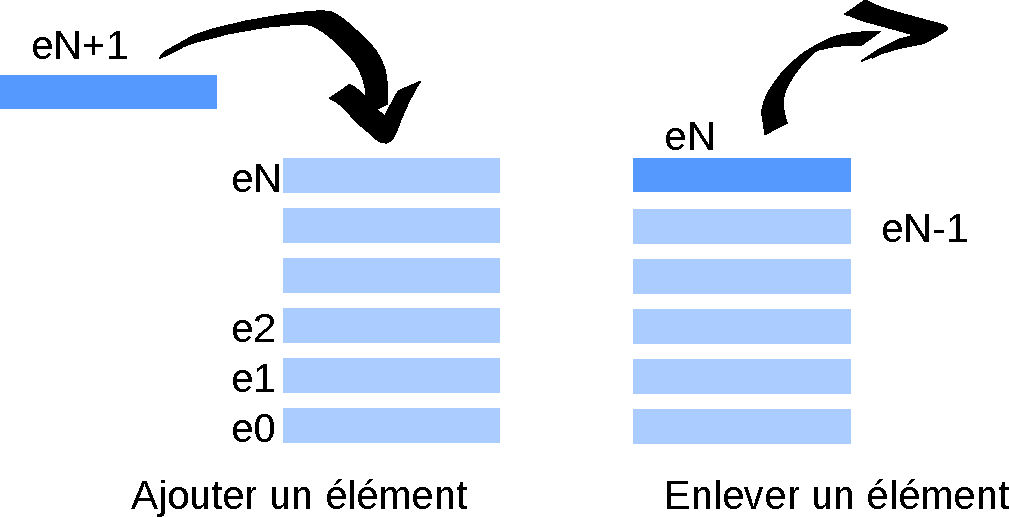
\includegraphics[width=0.6\linewidth]{images/pile.pdf}
	    \end{center}
\end{frame}

\begin{frame}[fragile=singleslide]
	\frametitle{Exemple - Calcul de $n!$}
	
	\begin{block}{Expression mathématique sous forme récursive}
    $$    fact(n)= 
    \begin{cases}
        n \times fact(n-1)~, & \text{si } n > 0\\
        0~,              & \text{sinon.}
    \end{cases}
	$$
    \end{block}
	
    \begin{block}{Implémentation récursive en C++}
		\begin{minted}{cpp}
int fact(int n){
    if(n <= 0){
    	// Cas de base
        return 1;
    } else {
    	// Formule de récurrence
        return n * fact(n - 1);
    }
}
		\end{minted}
    \end{block}

\end{frame}

\begin{frame}[fragile=singleslide]
	\frametitle{Tableaux dynamiques}

	\begin{block}{Le tas}
		Le tas est une autre zone mémoire (différente de la pile) qui est accessible dynamiquement à la demande du programme.
	\end{block}

	\begin{minted}{cpp}
...
int taille = 1e7; // taille pas forcément constante

int* tab = new int[taille]; // réserve la place dans le tas
...
// utilisation du tableau comme un tableau classique
...

delete[] tab; // désalloue la mémoire occupée dans le tas
		\end{minted}
	
	\begin{itemize}
		\item La taille du tableau n'a pas à être connu au moment de la compilation,
        \item Le tableau peut changer de taille au cours du programme,
		\item \textbf{Il ne faut pas oublier le \texttt{delete [] nom}}.
	\end{itemize}
\end{frame}

\section{Tableaux 2D}

\begin{frame}[fragile=singleslide]{Tableaux 2D}

	Les tableaux 2D de taille constante sont autorisés en C++.

	\begin{minted}{cpp}
// Déclaration d'un tableau 2D
double tab2D[5][3];
// Accès aux éléments
for(int i=0; i<5; i++){
    for(int j=0; j<3; j++){
	    tab2D[i][j] = i*j;
        // ATTENTION : pas de "tab2D[i,j]"
        cout << tab2D[i][j] << " ";
    }
    cout << endl;
}
// Initialisation
int t2D[2][3] = {{1,2,3},{4,5,6}};
	\end{minted}
En fait, \mintinline{cpp}{int t2D[2][3];} est un tableau de tableaux : \mintinline{cpp}{t2D[0]} et \mintinline{cpp}{t2D[1]} sont des tableaux de 3 cases.
\end{frame}

\begin{frame}[fragile=singleslide]{Tableaux 2D et fonctions}
    On peut utiliser les tableaux 2D dans les fonctions, mais il faut en spécifier les dimensions dans la signature de la fonction\,:
    \begin{minted}{cpp}
void init(int t[2][3], int val){
// Passage implicite par référence
    for(int i=0; i<2; i++){
        for(int j=0; j<3; j++){
            t[i][j] = val;
        }
    }
}

void f(){
    int tab[2][3];
    init(tab, 0); // appel de la fonction sur la variable tab
}
        
    \end{minted}
\end{frame}

\begin{frame}[fragile=singleslide]{Limitations}
	\begin{alertblock}{Fonctions génériques}
    Cas 1D : il est possible de faire des fonctions génériques
    \begin{minted}{cpp}
void init(int t[], int taille, int val){
    for(int i=0; i<taille; i++){
        t[i] = val;
    }
}
    \end{minted}
    Cas 2D : ce n'est pas possible
    \begin{minted}{cpp}
void init(int t[][], int rows, int cols, int val){...} //ERREUR        
    \end{minted}
    \end{alertblock}
    
    $\rightarrow$ Réécriture de code ? une fonction pour chaque taille de tableau ?
\end{frame}

\begin{frame}{Solution}
    On utilise des toujours des tableaux à 1 dimension.
    \begin{center}
        \begin{minipage}{0.2\linewidth}
        \begin{flushright}
        \begin{tabular}{|c|c|}
            \hline
            a & b\\
            \hline
            c & d\\
            \hline
            e & f\\
            \hline
        \end{tabular}
    \end{flushright}
        \end{minipage}
        \begin{minipage}{0.07\linewidth}
             \centering
        $\longrightarrow$
        \end{minipage}
        \begin{minipage}{0.5\linewidth}
        \begin{tabular}{|c|c|c|c|c|c|}
            \hline
            a & c & e &
            b & d & f \\
            \hline
        \end{tabular}
        \end{minipage}
    \end{center}
    Cette solution permet de gérer autant de dimension qu'on le souhaite.
\end{frame}

\begin{frame}{Parcourir un tableau 2D $\rightarrow$ 1D}
	On utilise soit le \textbf{parcours en lignes}, soit le \textbf{parcours en colonnes}.
    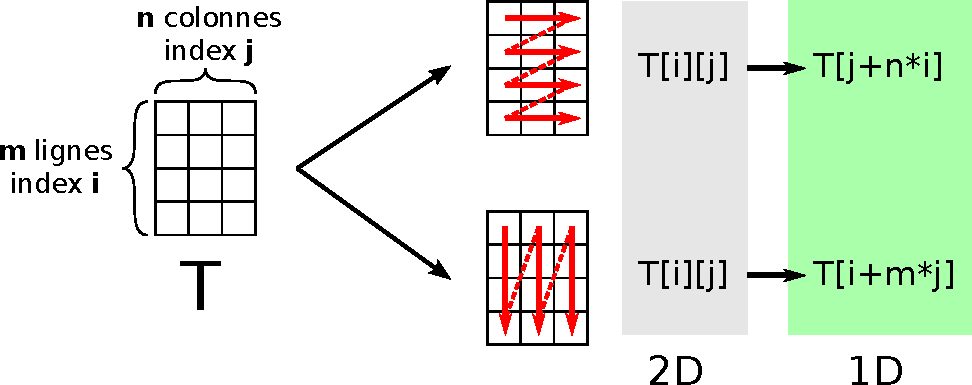
\includegraphics[width=\linewidth]{images/parcours.pdf}
\end{frame}

\begin{frame}[fragile=singleslide]{Utilisation dans les fonctions}
    Il est désormais possible d'utiliser des fonctions génériques.
    \begin{minted}{cpp}
        
double fill(double mat[], int rows, int cols, double val){
    for(int i=0; i<rows; i++){
        for(int j=0; j<cols; j++){
            mat[j+cols*i] = val;
        }
    }
}

void prod_mat_vec(double mat[], int rows, int cols, double vec[], double sol[]){
    for(int i=0; i<rows; i++){
        sol[i] = 0;
        for(int j=0; j<cols; j++){
            sol[i] += mat[j+cols*i]*vec[j];
        }
    }
}
        
    \end{minted}
\end{frame}

\section{Allocation dynamique}

\begin{frame}[fragile=singleslide]{Tableaux de taille variable}
    \begin{block}{Allocation dynamique et tableaux 2D}
        Pas de possibilité de faire des tableaux 2D avec allocation dynamique (tableaux de taille variable).
    \end{block}
    \begin{block}{Solution}
        On fait des tableaux 1D, comme précédemment.
    \end{block}
    \begin{minted}{cpp}
        
int m =...;
int n =...;
double* A = new double[m*n];
double* x = new double[m];
double* y = new double[n];
...
void prod_mat_vec(A,m,n,x,y);
...
delete[] A;
delete[] x;
delete[] y;
        
    \end{minted}
\end{frame}

\begin{frame}{Pointeurs}
    \begin{block}{Définition}
        Un \textbf{pointeur} est une variable qui stocke une adresse vers une zone mémoire (tableau ou variable) dans la pile ou dans le \textbf{tas}.
    \end{block}
    \begin{center}
    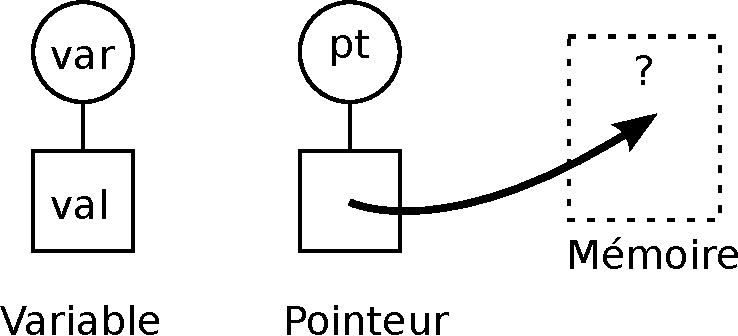
\includegraphics[width=0.8\linewidth]{images/var_pointeur.pdf}
    \end{center}
\end{frame}

\begin{frame}[fragile=singleslide]{Déclarer un pointeur}
    On utilise le caractère \texttt{*}.
    \begin{minted}{cpp}
        
int* ptr; // un pointeur vers un entier
        
    \end{minted}
    Pour récupérer l'adresse d'une variable on utilise le \texttt{\&}
    \begin{minted}{cpp}
        
int* ptr; // un pointeur vers un entier
int test = 10;
ptr = &test; // le pointeur redirige vers test
        
    \end{minted}
    \begin{center}
        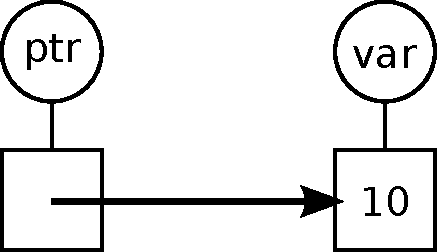
\includegraphics[width=0.27\linewidth]{images/ptr.pdf}
    \end{center}
\end{frame}

\begin{frame}{Pointeurs et mémoire}
    L'intérêt d'utiliser des pointeurs avec des variables classiques est limité.

    \begin{block}{Des pointeurs pour le tas}
        Les pointeurs sont la porte d'entrée vers le tas (la mémoire de l'ordinateur).
    \end{block}
    \begin{itemize}
        \item Créer une variable dans le tas : \textbf{\texttt{new}}
        \item Supprimer une variable dans le tas : \textbf{\texttt{delete}}
    \end{itemize}
\end{frame}

\begin{frame}{Pointeurs et tableaux}
\centering
\includegraphics<1>[width=\linewidth]{images/tableaux_tas_01.pdf}
\includegraphics<2>[width=\linewidth]{images/tableaux_tas_02.pdf}
\includegraphics<3>[width=\linewidth]{images/tableaux_tas_03.pdf}
\includegraphics<4>[width=\linewidth]{images/tableaux_tas_04.pdf}
\includegraphics<5>[width=\linewidth]{images/tableaux_tas_05.pdf}
\end{frame}

\begin{frame}{Pointeurs et fonctions}
\begin{block}{Modifier la variable / tableau désigné par le pointeurs}
    \begin{itemize}
        \item Pas besoin de passage par référence : on ne modifie pas le pointeur (l'adresse), seulement les valeurs stockées dans la zone de la mémoire désignées par le pointeur.
        \item On peut utiliser les fonctions créées pour les tableaux statiques.
    \end{itemize}
\end{block}

\begin{center}
    \vspace{-0.2cm}
    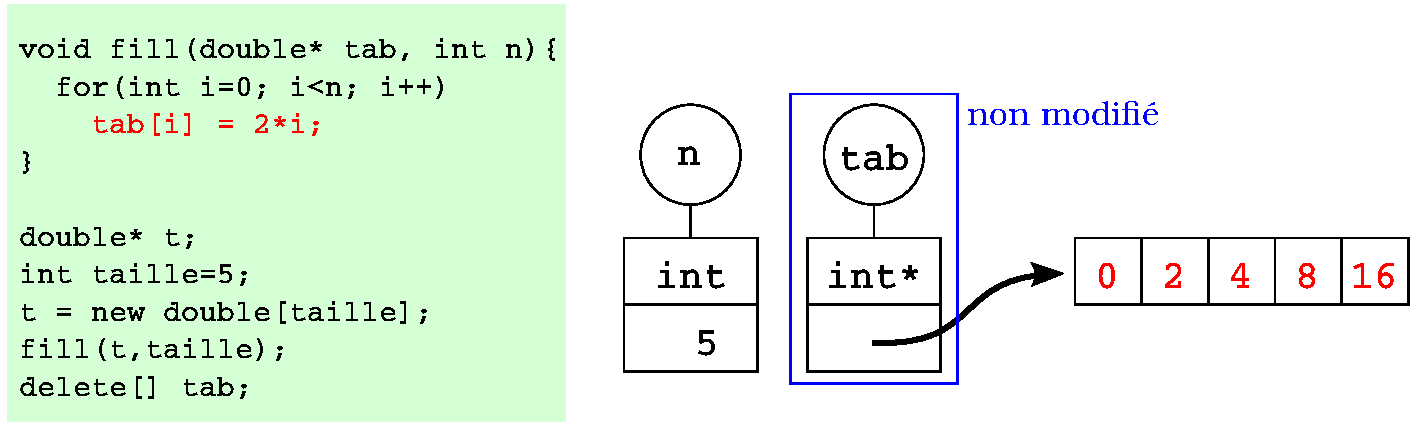
\includegraphics[width=\linewidth]{images/function_ptr_1.pdf}
\end{center}
\end{frame}

\begin{frame}{Pointeurs et fonctions}
\begin{block}{Modifier le pointeur}
    \begin{itemize}
    \item Il faut faire un passage par référence : on modifie l'adresse stockée par le pointeur.
    \end{itemize}
\end{block}
\begin{center}
\includegraphics<1>[width=\linewidth]{images/function_ptr_2_01.pdf}
\includegraphics<2>[width=\linewidth]{images/function_ptr_2_02.pdf}
\includegraphics<3>[width=\linewidth]{images/function_ptr_2_03.pdf}
\includegraphics<4>[width=\linewidth]{images/function_ptr_2_04.pdf}
\includegraphics<5>[width=\linewidth]{images/function_ptr_2_05.pdf}
\includegraphics<6>[width=\linewidth]{images/function_ptr_2_06.pdf}
\includegraphics<7>[width=\linewidth]{images/function_ptr_2_07.pdf}
\includegraphics<8>[width=\linewidth]{images/function_ptr_3_01.pdf}
\includegraphics<9>[width=\linewidth]{images/function_ptr_3_02.pdf}
\includegraphics<10>[width=\linewidth]{images/function_ptr_3_03.pdf}
\includegraphics<11>[width=\linewidth]{images/function_ptr_3_04.pdf}
\includegraphics<12>[width=\linewidth]{images/function_ptr_3_05.pdf}
\includegraphics<13>[width=\linewidth]{images/function_ptr_3_06.pdf}
\includegraphics<14>[width=\linewidth]{images/function_ptr_3_07.pdf}
\end{center}
\end{frame}

\begin{frame}{Egalité de pointeurs}
    L'égalité de pointeurs est autorisée.

    \begin{alertblock}{Attention}
        \begin{itemize}
            \item Il y a des risques de fuite de mémoire
            \item Deux pointeurs égaux renvoient au même espace mémoire
            \item Il n'y a pas création d'un nouveau tableau
        \end{itemize}
    \end{alertblock}

    \begin{center}
        \includegraphics<1>[width=\linewidth]{images/egalite_ptr_1.pdf}
        \includegraphics<2>[width=\linewidth]{images/egalite_ptr_2.pdf}
        \includegraphics<3>[width=\linewidth]{images/egalite_ptr_3.pdf}
    \end{center}
\end{frame}

\begin{frame}[fragile=singleslide]{Egalité de pointeurs 2}
    Pour copier un tableau, il faut le faire terme à terme.
    \begin{minted}{cpp}
        
double* t,s;
int n = 100;
t = new double[n];

...

// copie du tableau
s = new double[n]; // allocation de la memoire
for(int i=0; i<n; i++){
    s[i] = t[i]; // recopie terme a terme
}
...
delete[] t; // liberation tableau t
delete[] s; // liberation tableau s
        
    \end{minted}
\end{frame}

\section{Structures et allocation dynamique}

\begin{frame}[fragile=singleslide]{Des tableaux dans des structures}
    Il est possible d'utiliser des tableaux dynamiques dans les structures.
    \begin{alertblock}{Attention}
        Surtout pas de tableaux statiques.
    \end{alertblock}
    \begin{minted}{cpp}
        
struct Vect{
    int taille; // la taille
    double* t; // le tableau, ne pas allouer
               // dans la declaration de la structure
};
        
    \end{minted}

\end{frame}

\begin{frame}[fragile=singleslide]{Structures et allocation dynamique}
    \begin{minipage}{0.48\linewidth}
    \vspace{-4em}
	\begin{minted}{cpp}
// Vect.h
struct Vect{
    int n; // taille
    double* t; // tableau
};

void init(Vect& v);

void cree(Vect& v, int n);

void detruit(Vect& v);

void remplit(Vect& v, double val);

void copie(Vect& v, Vect o);

Vect operator+(Vect v1, Vect v2);
	\end{minted}
    \end{minipage}
    \begin{minipage}{0.48\linewidth}
        \begin{minted}{cpp}
// Vect.cpp
#include "Vect.h"
void init(Vect& v){
    v.n = 0;
}

void cree(Vect& v, int n){
    assert(n > 0);
    v.n = n;
    v.t = new double[v.n];
}

void detruit(Vect& v){
    if(v.taille > 0){
        v.taille = 0;
        delete[] v.t;
    }
}

void remplit(Vect& v, double val){
    for(int i=0; i<v.n; i++){
        v.t[i] = val;
    }
}
        \end{minted}
    \end{minipage}
\end{frame}

\begin{frame}[fragile=singleslide]{Structures et allocation dynamique}
    \begin{minipage}{0.48\linewidth}
        \vspace{-3em}
        \begin{minted}{cpp}
// Vect.h
struct Vect{
    int n; // taille
    double* t; // tableau
};

void init(Vect& v);

void cree(Vect& v, int n);

void detruit(Vect& v);

void remplit(Vect& v, double val);

void copie(Vect& v, Vect o);

Vect operator+(Vect v1, Vect v2);
        \end{minted}
    \end{minipage}
    \begin{minipage}{0.50\linewidth}
        \begin{minted}{cpp}
// Vect.cpp
#include "Vect.h"
void copie(Vect& v, Vect o){
    detruit(v);
    cree(v, o.taille);
    for(int i=0;i<v.n;i++)
        v.t[i] = o.t[i];
}

Vect operator+(Vect v1, Vect v2){
    assert(v1.n == v2.n);
    Vect v;
    cree(v, v1.n);
    for(int i=0;i<v.n; i++)
        v.t[i] = v1.t[i]+v2.t[i];
    return v;
}
        \end{minted}
    \end{minipage}
\end{frame}

\begin{frame}[fragile=singleslide]{Structures et allocation dynamique}
    \begin{minipage}{0.48\linewidth}
    \vspace{-3em}
        \begin{minted}{cpp}
// Vect.h
struct Vect{
    int n; // taille
    double* t; // tableau
};

void init(Vect& v);

void cree(Vect& v, int n);

void detruit(Vect& v);

void remplit(Vect& v, double val);

void copie(Vect& v, Vect o);

Vect operator+(Vect v1, Vect v2);
        \end{minted}
    \end{minipage}
    \begin{minipage}{0.48\linewidth}
        \begin{minted}{cpp}
// main.cpp
#include "Vect.h"

int main(){
    Vect v1,v2;
    init(v1);
    init(v2);

    cree(v1, 10);
    remplit(v1, 5.6);

    copie(v2, v2);

    Vect v3 = v1 + v2;

    detruit(v1);
    detruit(v2);
    detruit(v3);
    return 0;
}
        \end{minted}
    \end{minipage}
\end{frame}

\section{Boucles, break et continue}

\begin{frame}[fragile=singleslide]{break}

    L'instruction \textbf{\texttt{break}} permet de sortir d'une boucle.
    \vspace{-0.1cm}
    \begin{minted}{cpp}
        
for(int i=0; i<n; i++){
    bool b = f(i);
    if(!b) break; // sort de la boucle si b est faux
}
        
    \end{minted}

    \vspace{-0.1cm}
Pour sortir de boucles imbriquées, il faut utiliser des booléens.
    \vspace{-0.1cm}
\begin{minipage}{0.47\linewidth}
    \begin{minted}{cpp}   
bool stop = false;
for(int i=0; i<n; i++){
    for(int j=0; j<m; j++){
        if(i*j > 100){
            stop = true;
            break;
        }
    }
    if(stop) break;
}
    \end{minted}
\end{minipage}
\hfill
\begin{minipage}{0.47\linewidth}
    \begin{minted}{cpp}   
bool go = true;
for(int i=0; i<n && go; i++){
    for(int j=0; j<m && go; j++){
        if(i*j > 100){
            go = false;
        }
    }
}     
    \end{minted}
\end{minipage}

\end{frame}

\begin{frame}[fragile=singleslide]{continue}
L'instruction \texttt{\textbf{continue}} permet de passer à l'itération suivante dans une boucle (sans exécuter ce qui se trouve après le \texttt{\textbf{continue}}).

\begin{minted}{cpp}
    
int i=1;
while(i< 1000){
    i++;
    if(i%2 == 1)
        continue;
    cout << i << " est pair" << endl;
}
    
\end{minted}

\end{frame}

\section{TP du jour}

\begin{frame}{Le TP}

\begin{minipage}{0.47\linewidth}
    Manipulation d'images.

    \begin{itemize}
        \item Tableaux 2D en allocation dynamique
        \item Opérations courantes sur les images (flou, inversion, contraste...)
        \item Manipulation de structure et d'allocation dynamique
    \end{itemize}
\end{minipage}
\hfill
\begin{minipage}{0.47\linewidth}
    \centering
    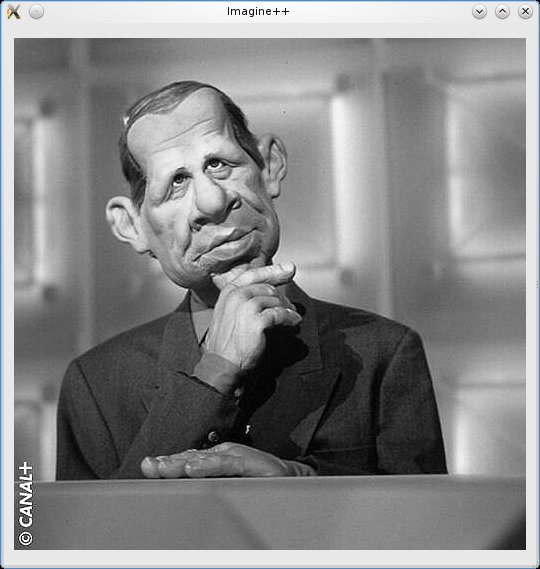
\includegraphics[width=0.47\linewidth]{images/ppd_2.png}
    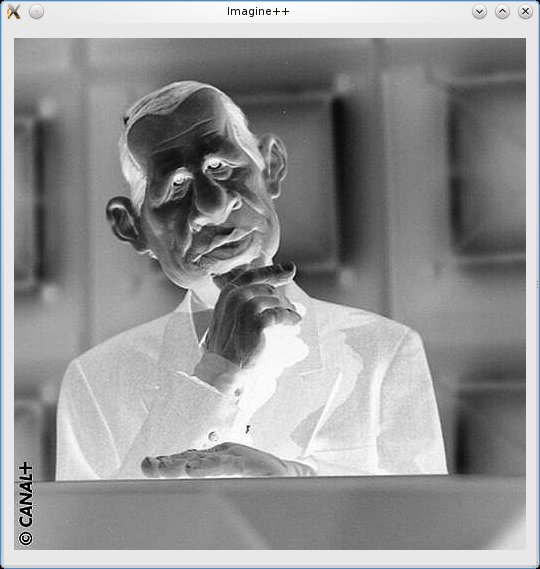
\includegraphics[width=0.47\linewidth]{images/ppd.png}\\
    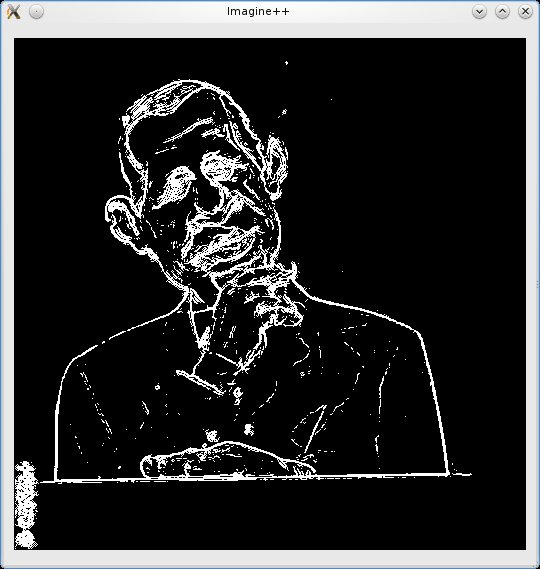
\includegraphics[width=0.47\linewidth]{images/ppd_3.png}
    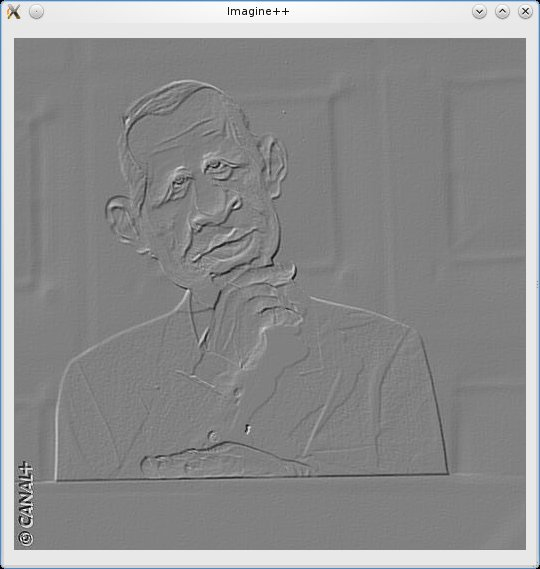
\includegraphics[width=0.47\linewidth]{images/ppd_4.png}
\end{minipage}

\end{frame}

\end{document}


